\documentclass[a5paper, 8pt,american]{book}
\usepackage[tmargin=1in, bmargin=1in]{geometry}

%\documentclass[12pt]{report}
%\usepackage[a4paper]{geometry}
%\geometry{left=2.75cm,right=2.75cm, top=3cm, bottom=3cm}

\usepackage{amssymb,amsmath, amsfonts,eurosym,graphicx,caption,color,setspace,sectsty,comment,footmisc,caption,array,hyperref, subcaption, float, lscape, booktabs, longtable, multirow, rotating, wrapfig, pdflscape, tabu, threeparttablex, threeparttable, makecell, xcolor, authblk, natbib, bbm, comment, dcolumn, pdflscape, appendix, tabularx, fancyhdr, etoolbox, lipsum}
\usepackage[sc]{mathpazo}
\linespread{1.0}
\usepackage[T1]{fontenc}

%\definecolor{fairpurple}{RGB}{108, 32, 50}
\definecolor{fairpurple}{RGB}{0, 0, 0}
\definecolor{fairpink}{RGB}{204, 48, 122}
\definecolor{fairorange}{RGB}{231, 86, 66}
\definecolor{fairgray}{RGB}{171, 172, 176}
\hypersetup{colorlinks,citecolor=fairpurple, filecolor=fairorange, linkcolor=fairpurple, urlcolor=fairpurple}
\let\svthefootnote\thefootnote
\newcommand\freefootnote[1]{%
  \let\thefootnote\relax%
  \footnotetext{#1}%
  \let\thefootnote\svthefootnote%
}

% Set font size of chapter titles (set to be used with abstract on same page)
\chaptertitlefont{\large}

% Header style for main part (sets name of section on odd-numer pages, chapter number on even-number pages, and no header - only page number - in Introduction chapter).
\pagestyle{fancy}
\fancypagestyle{main}{%
	\fancyhead[EL, OR]{\thepage}%
	\fancyhead[ER]{\ifnum \value{chapter}>0 \textsl{CHAPTER \thechapter}\fi}%
	\fancyhead[OL]{\ifnum \value{chapter}>0 \textsl{\rightmark}\fi}%
	\renewcommand{\headrulewidth}{0pt}%
	\fancyfoot{}%
}
% Header style for beginning ("frontmatter")
\fancypagestyle{plain}{%
  \fancyhf{}%
  \fancyfoot[C]{\thepage}%
  \renewcommand{\headrulewidth}{0pt}%
  \renewcommand{\footrulewidth}{0pt}%
}
% Assign the respective header style to the correct part of book
\appto\frontmatter{\pagestyle{plain}}
\appto\mainmatter{\pagestyle{main}}

% Appendix in TOC
\AtBeginEnvironment{subappendices}{%
  \addtocontents{toc}{\protect\addvspace{1pt}\textcolor{fairpurple}{Appendices}}
}
\makeatletter
\patchcmd{\@chapter}{\protect\numberline{\thechapter}#1}
{\@chapapp~\thechapter: #1}{}{}
\makeatother

% Let space from bottom to text vary page by page
\raggedbottom

% Show only sections (not subsections) in ToC
\setcounter{tocdepth}{1}

\begin{document}

\frontmatter
\title{\huge Essays on Some Economic Topic}
\author{\Large Firstname Lastname \vspace{-0.4cm}}
\affil{Some School of Economics \vspace{-0.25cm}}
\date{}
\maketitle

\begin{onehalfspace}
\setcounter{page}{0}
\chapter*{Acknowledgements}  

% Here goes your acknowledgments, delete lipsum command and enter your text
\lipsum[1-5] \\

\begin{flushright}
    \textit{Firstname Lastname} \\
    Somewhere, June 2023\\
\end{flushright}



\end{onehalfspace}

\begin{singlespace}
    \tableofcontents
\end{singlespace}

\begin{onehalfspace}
\mainmatter
\chapter*{Introduction}
\addcontentsline{toc}{chapter}{Introduction} 

\lipsum[1-1]

\citep{bertrand2021improving}

\begin{figure}[!htb]
    \begin{center}
    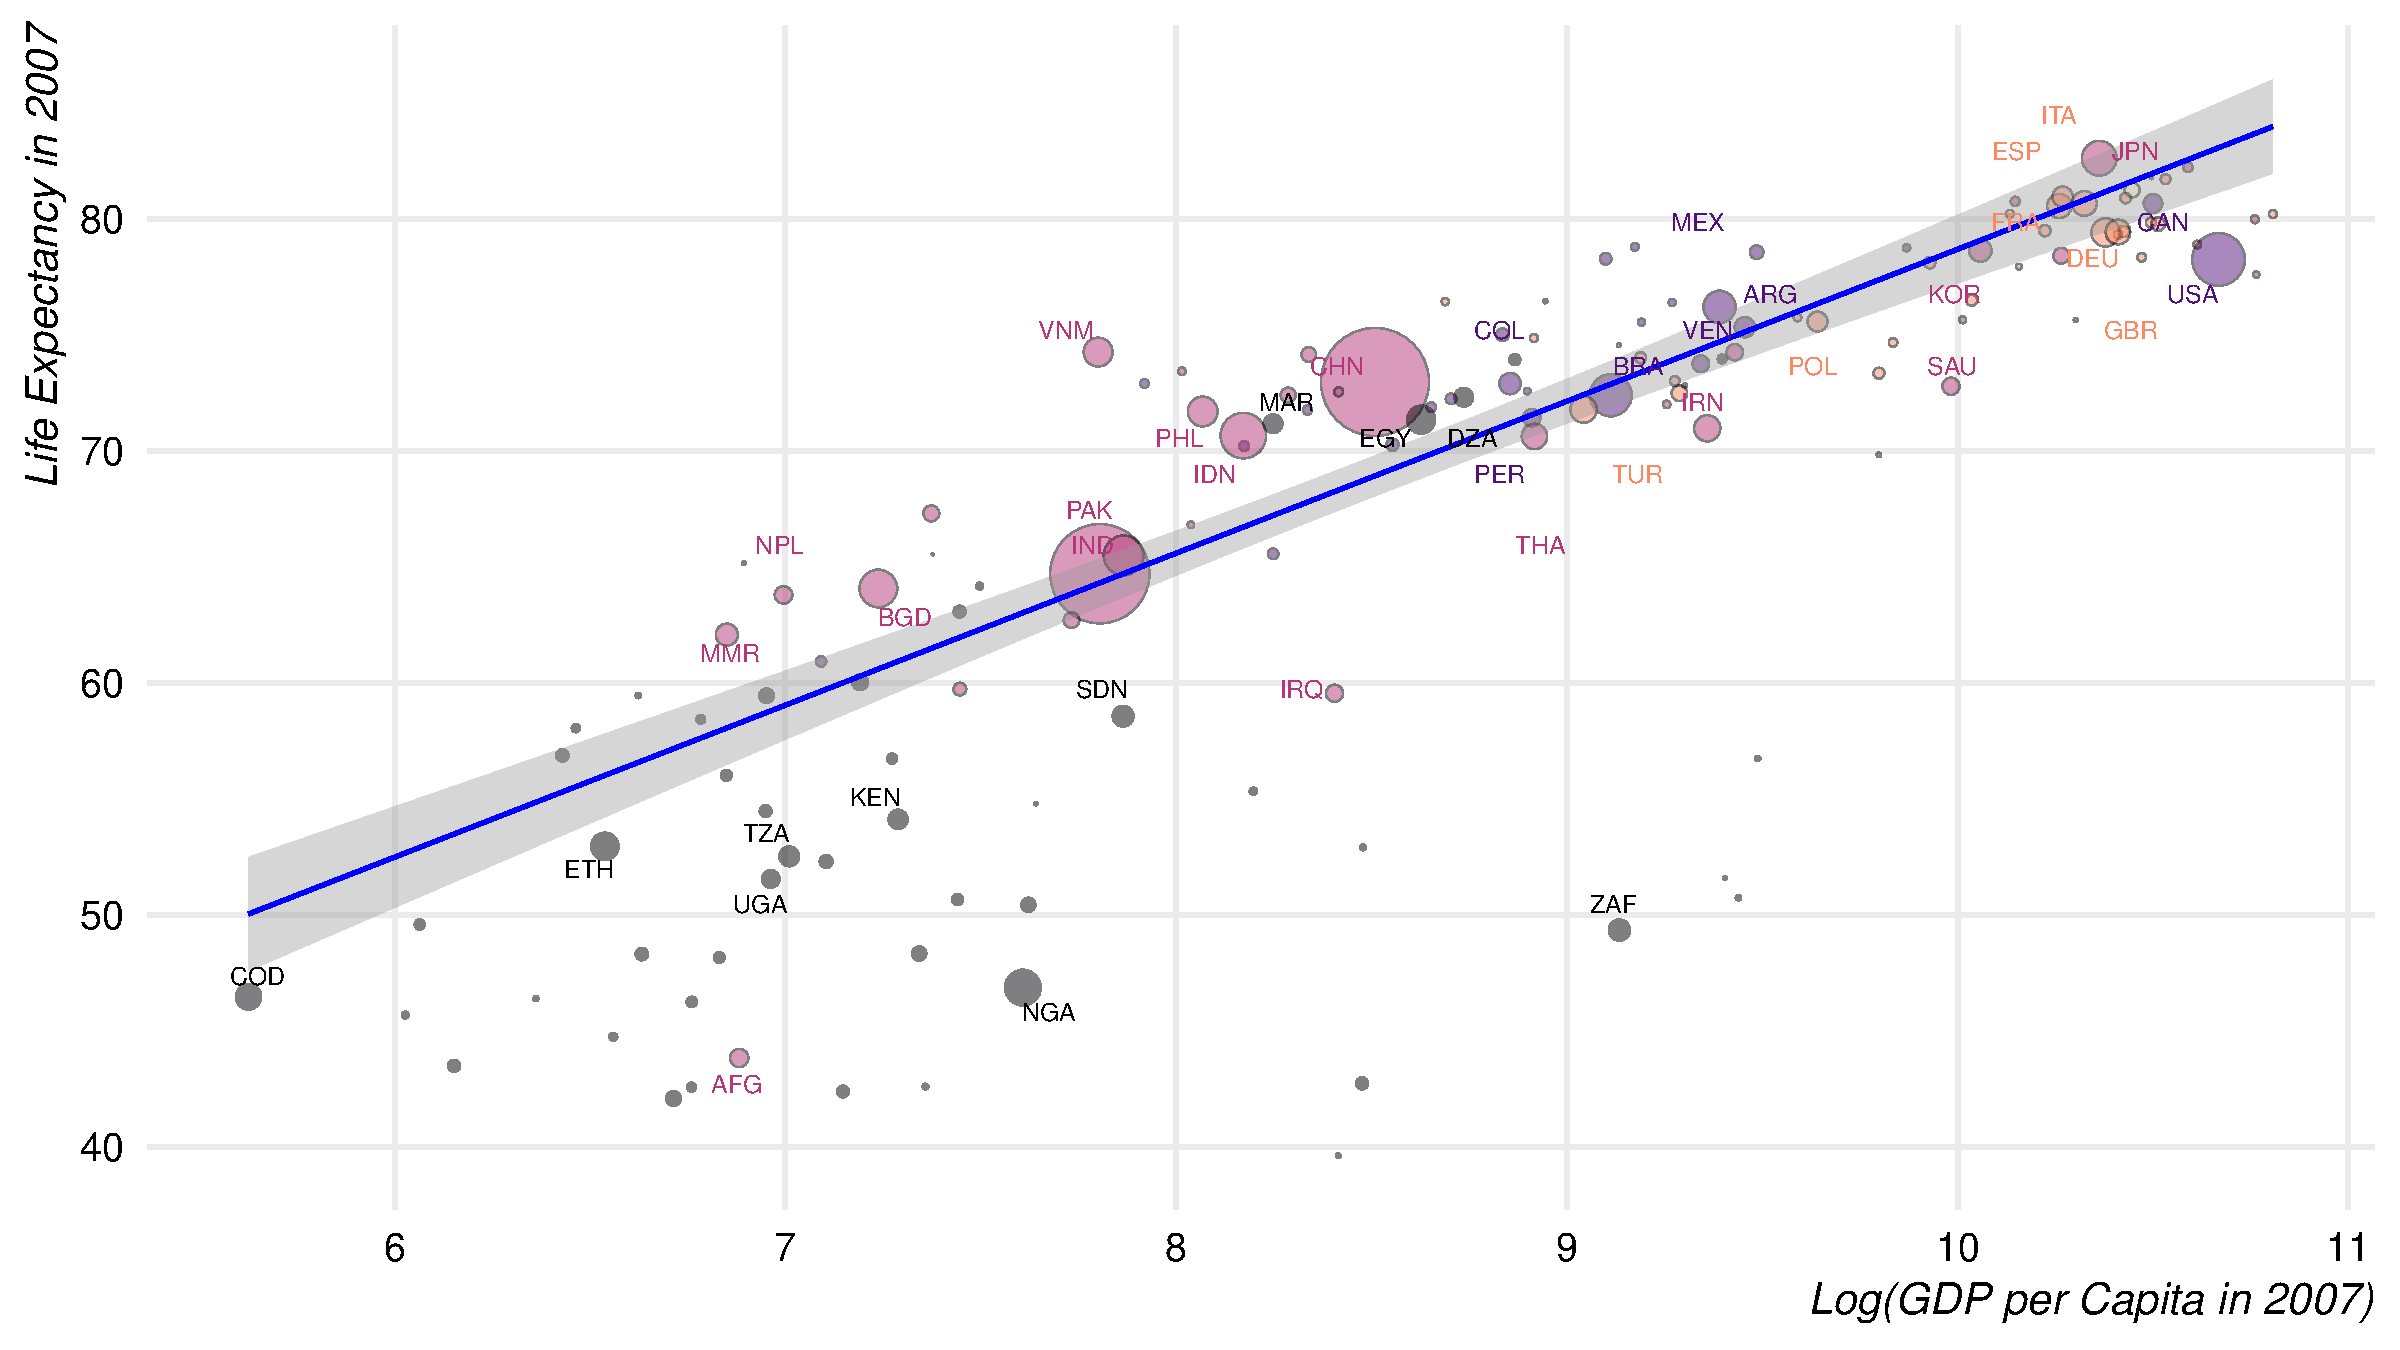
\includegraphics[width=\linewidth]{figures/gapminder_plot.pdf}
    \end{center}
    \caption{Association between GDP per Capita and Life-Expectancy in 2007.}
    \label{fig:gapminder}
    \begin{singlespace}
        \scriptsize{\textit{Note:} The figure plots the logarithm of GDP per capita on the x-axis and life-expectancy on the y-axis. The size of the bubbles indicates the population size of countries and the colour indicates the continent of the country. ISO labels are included for countries with a population above 25 Million. The blue line is fitted using a linear regression weighted by population size.}
    \end{singlespace}
\end{figure}

\lipsum[1-6] 
\citet{black2013under}


\chapter{Title of First Paper}\freefootnote{Here can go your thanks and other footnotes. }
\vspace{-1cm}

\begin{small} 
    \begin{quote}
        \textbf{Abstract:} \lipsum[1-1]
    \end{quote}
\end{small}
\newpage

\setcounter{footnote}{0} 
\section{Section 1} \label{seclong:label3}

\lipsum[1-6]

\section{Section 2} \label{seclong:label2}

\lipsum[1-10]


\newpage
\thispagestyle{empty}
\section*{Appendices}

\begin{subappendices}
    \setcounter{table}{0}
    \renewcommand{\thetable}{A\arabic{table}}
    \setcounter{figure}{0}
    \renewcommand{\thefigure}{A\arabic{figure}}

    \section{Some Tables} \label{app:tables}
    


    \section{Some Figures} \label{app:figures}

    





\end{subappendices}

\chapter{Title of Second Paper}\freefootnote{Here can go your thanks and other footnotes. }
\vspace{-1cm}

\begin{small}
    \begin{quote}
        \textbf{Abstract:} \lipsum[1-1]
    \end{quote}
\end{small}
\newpage

\setcounter{footnote}{0} 
\section{Section 1} \label{seclong:label3}

\lipsum[1-6]

\section{Section 2} \label{seclong:label2}

\lipsum[1-10]


\newpage
\thispagestyle{empty}
\section*{Appendices}

\begin{subappendices}
    \setcounter{table}{0}
    \renewcommand{\thetable}{A\arabic{table}}
    \setcounter{figure}{0}
    \renewcommand{\thefigure}{A\arabic{figure}}

    \section{Some Tables} \label{app:tables}
    

    \section{Some Figures} \label{app:figures}

    





\end{subappendices}
\newpage

\chapter{Title of Third Paper}\freefootnote{Here can go your thanks and other footnotes. }
\vspace{-1cm}

\begin{small}
    \begin{quote}
        \textbf{Abstract:} \lipsum[1-1]
    \end{quote}
\end{small}
\newpage

\setcounter{footnote}{0} 
\section{Section 1} \label{seclong:label3}

\lipsum[1-6]

\section{Section 2} \label{seclong:label2}

\lipsum[1-10]


\newpage
\thispagestyle{empty}
\section*{Appendices}

\begin{subappendices}
    \setcounter{table}{0}
    \renewcommand{\thetable}{A\arabic{table}}
    \setcounter{figure}{0}
    \renewcommand{\thefigure}{A\arabic{figure}}

    \section{Some Tables} \label{app:tables}
    

    \section{Some Figures} \label{app:figures}

    





\end{subappendices}

\end{onehalfspace}

\newpage
\addcontentsline{toc}{chapter}{Bibliography}

% make sure to have the aea.bst file in the same folder as your main tex-file
\bibliographystyle{aea}

% path to your bib-file (without .bib extension)
\bibliography{/home/rene/Dropbox/NHH/Literature/Literature_database}








\end{document}
